\chapter{Introduction}
\label{chap:introduction}


% =================================================================
% 1.1 Fetal Biometry and Clinical Motivation
% =================================================================

\section{Fetal Biometry and Clinical Motivation}
\label{sec:intro-motivation}

Fetal biometry is the routine ultrasound measurement of fetal
anatomical structures used to estimate gestational age and monitor
fetal growth throughout pregnancy \parencite{salomon2019isuog}. This
thesis considers five landmark-defined linear measurements across
three anatomical standard planes
\parencite{divece2025multicentre}: the biparietal diameter (\BPD)
and occipito-frontal diameter (\OFD) on the head plane, the
transverse abdominal diameter (\TAD) and anteroposterior abdominal
diameter (\APAD) on the abdominal plane, and femur length (\FL) on
the femur plane. Each measurement is determined by a pair of
anatomical landmarks placed by the sonographer on a standard 2D
ultrasound image. Representative examples of the five measurements
and their landmark annotations are shown in
\Cref{fig:fetal-biometry-measurements}.

\begin{figure}[!ht]
\centering
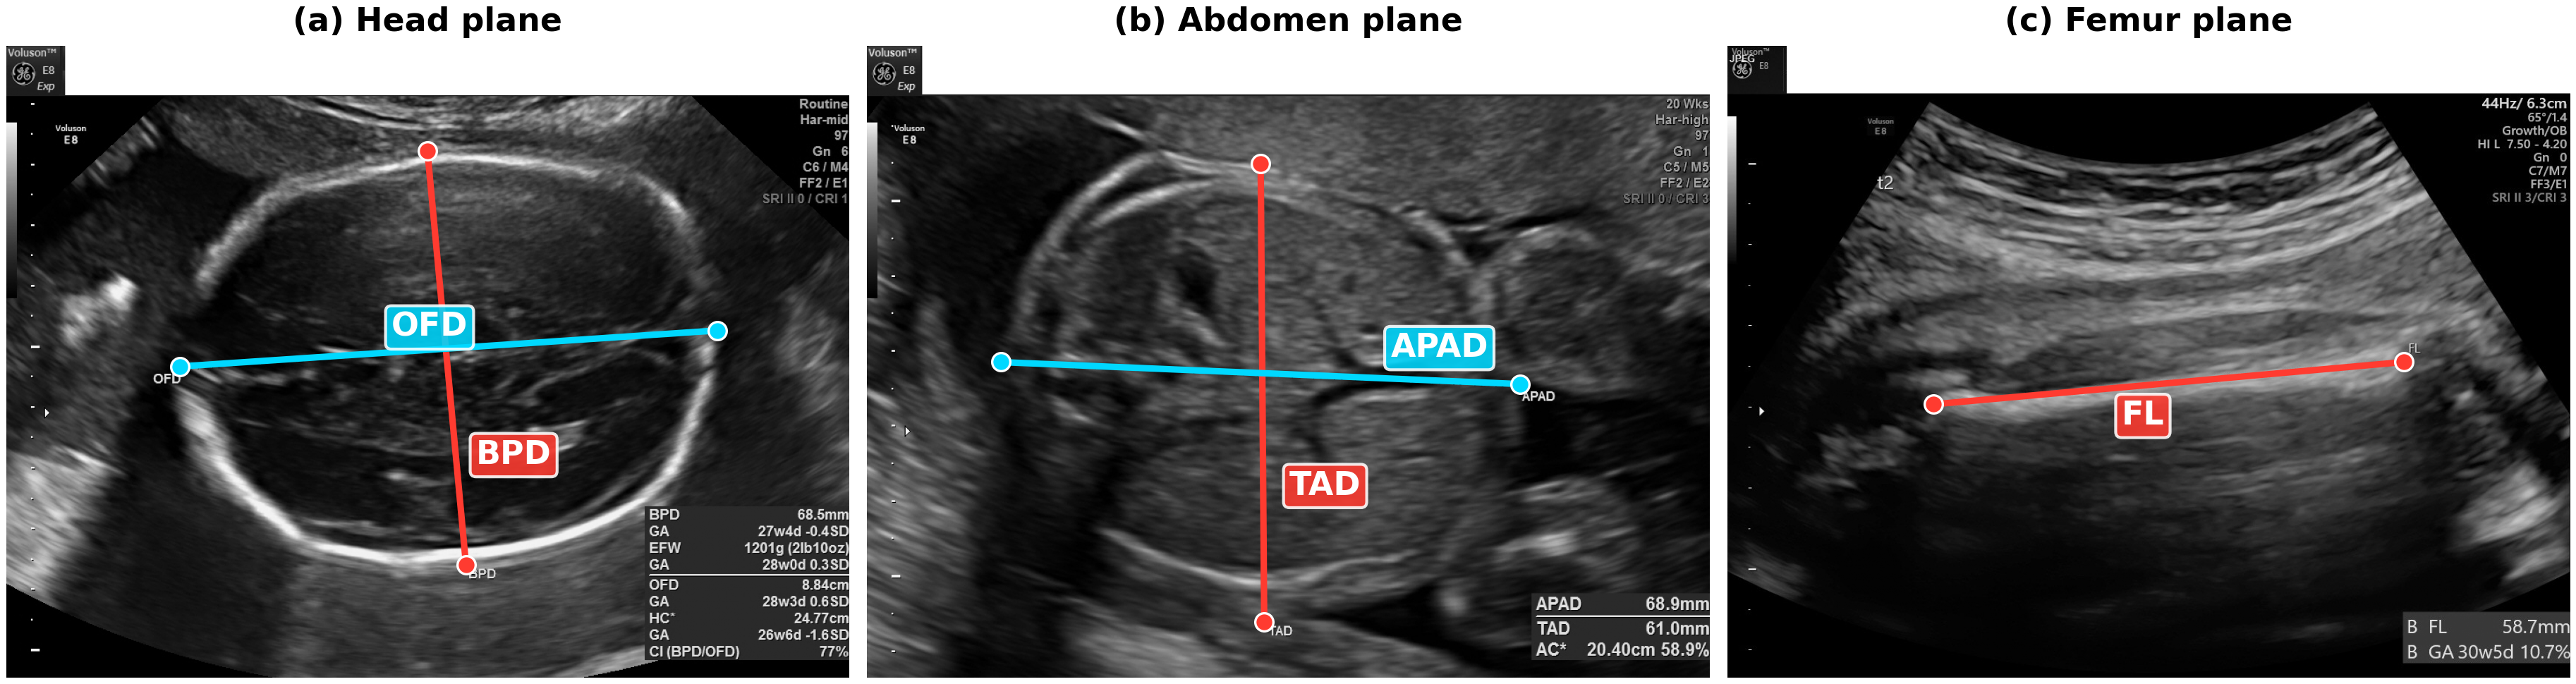
\includegraphics[width=\textwidth]
  {figures/fetal_biometry_measurements.png}
\caption{Representative fetal ultrasound images showing the five
biometric measurements considered in this thesis across the three
standard planes: (a) BPD and OFD on the head plane, (b) TAD and
APAD on the abdominal plane, and (c) FL on the femur plane. Each
measurement is defined by two anatomical landmarks, which constitute
the localisation targets in this study. Images and ground-truth
annotations are from the released UCL subset of the Multicentre
Fetal Biometry dataset \parencite{divece2025multicentre}.}
\label{fig:fetal-biometry-measurements}
\end{figure}

Manual landmark placement is not perfectly reproducible. For related
fetal measurements, \textcite{sarris2012intra} reported absolute
95\% limits of agreement ranging from 4.9\% to 11.1\% for
inter-observer differences and from 3.0\% to 6.6\% for
intra-observer differences. This operator dependence provides a
direct motivation for automated landmark localisation. Given the
same image, an automated system could reduce the variability
introduced by repeated manual landmark placement, while leaving
errors associated with image acquisition and standard-plane
selection outside its scope.


% =================================================================
% 1.2 Automated Fetal Landmark Localisation and VFMs
% =================================================================

\section{Automated Fetal Landmark Localisation and Vision Foundation
Models}
\label{sec:intro-gap}

Recent work has increasingly applied deep learning to automated fetal
biometry. P{\l}otka et al.\ developed a deep-learning approach for
automated fetal biometric measurement
\parencite{plotka2022fuvai}, while Gao et al.\ investigated
landmark-focused prediction for fetal biometry
\parencite{gao2023endpoints}. A particularly relevant formulation is
provided by the Multicentre Fetal Biometry study, which casts
biometric measurement as paired landmark localisation and provides
the principal benchmark reproduced in this thesis
\parencite{divece2025multicentre}. Its HRNet-W18-based pipeline
incorporates Dynamic Orientation Determination (DOD) to resolve the
inherent ordering ambiguity of paired landmarks.

Convolutional landmark localisation has evolved from architectures
that repeatedly aggregate multi-scale context, such as stacked
hourglass networks \parencite{newell2016hourglass}, to
deconvolutional prediction heads such as SimpleBaseline
\parencite{xiao2018simple} and high-resolution representations such
as HRNet \parencite{sun2019hrnet}. Heatmap regression has been
successfully applied to fetal biometry, while coordinate-
classification methods such as RTMPose
\parencite{jiang2023rtmpose} provide a complementary paradigm for
precise keypoint localisation. Despite their different output
formulations, these methods still rely primarily on task-specific
supervised adaptation.

Self-supervised vision foundation models shift the problem from
learning visual representations largely from task-specific
annotations to adapting representations acquired at scale. DINOv2
\parencite{oquab2023dinov2} and DINOv3
\parencite{simeoni2025dinov3} learn general-purpose visual
representations from large image corpora through self-distillation,
without requiring manual annotations for pretraining. Such
representations are attractive for fetal ultrasound, where expert
landmark annotations are costly and labelled datasets are
comparatively limited. The remaining challenge is spatial: precise
fetal biometry requires the model to form landmark-specific
representations while retaining sufficient spatial detail for
accurate localisation. How best to adapt general-purpose foundation
model representations to this setting remains underexplored.


% =================================================================
% 1.3 QCLand and Research Questions
% =================================================================

\section{QCLand and Research Questions}
\label{sec:intro-approach}

To bridge this gap, this thesis introduces \textbf{QCLand}
(Query-Conditioned Landmark Localisation), a framework that adapts
pretrained vision representations through landmark-specific query
interaction and spatial decoding. Each fetal measurement is modelled
independently: a separate QCLand model is trained for each
measurement, with two learned landmark queries corresponding to its
two landmark channels. The queries are inserted into the backbone
token sequence, allowing self-attention to form landmark-specific
representations directly through interaction with the image tokens.
This query-in-encoder formulation is inspired by recent encoder-only
query architectures \parencite{kerssies2025eomt} and is adapted here
for two-landmark localisation.

A new spatial decoding head, DeconvHeadV2, converts the
query-conditioned representations into high-resolution landmark
heatmaps for precise localisation. The framework is instantiated with
two self-supervised backbones, yielding QCLand-DINOv2 and
QCLand-DINOv3.

The thesis addresses three research questions:

\begin{description}

\item[RQ1] Can a pretrained vision foundation model be effectively
adapted for precise fetal biometry landmark localisation through
landmark-query conditioning and spatial decoding?

\item[RQ2] Which architectural adaptations are most important for
converting foundation-model representations into accurate landmark
predictions?

\item[RQ3] How does the resulting framework perform across
different fetal measurements, backbone generations
(DINOv2 vs.\ DINOv3), and the UCL and Multicentre dataset
settings, relative to established baselines?

\end{description}

The final four-model comparison provides the primary evidence for
RQ1 and RQ3 by evaluating QCLand against HRNet-W18 and RTMPose-s
across all ten dataset--measurement settings. RQ2 is investigated
through the BPD model-development study, which traces the
architectural changes leading to the adopted QCLand configuration
and examines the relative importance of the evaluated modifications.


% =================================================================
% 1.4 Contributions
% =================================================================

\section{Contributions}
\label{sec:intro-contributions}

The main contributions of this thesis are:

\begin{itemize}

\item \textbf{QCLand: query-conditioned foundation-model adaptation
for fetal landmark localisation.}
QCLand adapts pretrained DINOv2 and DINOv3 representations through
learned landmark-query interaction and spatial decoding. Its central
architectural contribution, DeconvHeadV2, replaces the inherited
dot-product readout with an explicit spatial-processing path,
providing a route from general-purpose transformer representations
to precise landmark predictions.

\item \textbf{A systematic model-development study for spatial
landmark decoding.}
Controlled experiments on BPD examine the architectural and training
changes leading to the final configuration. Among the evaluated
architectural modifications, DeconvHeadV2 produces the largest
observed reduction in localisation error, while the study also
establishes the effects and remaining uncertainties associated with
multi-depth feature fusion, pixel-centre alignment, and geometric
augmentation.

\item \textbf{Evaluation across measurements, backbones, and dataset
settings.}
QCLand-DINOv2 and QCLand-DINOv3 are evaluated across five fetal
measurements on both the UCL and Multicentre datasets against locally
reproduced HRNet-W18 and RTMPose-s baselines. The comparison uses
matched input resolution, five predefined seeds, common image
subsets, original-image-space permutation-invariant \NME{}, and
paired statistical testing. A QCLand variant achieves the lowest mean
error in eight of the ten evaluations, supporting the framework's
competitiveness across anatomical measurements and dataset settings.

\end{itemize}


% =================================================================
% 1.5 Dissertation Roadmap
% =================================================================

\section{Dissertation Roadmap}
\label{sec:intro-structure}

\Cref{chap:background} establishes the clinical and technical
context. \Cref{chap:method} defines the QCLand architecture and
training components. \Cref{chap:experimental-setup} specifies the
datasets, evaluation metric, compared models, and statistical
protocol. \Cref{chap:results} presents the comparative and ablation
results, interprets their variation across measurements and dataset
settings, and discusses the study's limitations and implications.
\Cref{chap:conclusion} summarises the findings and identifies
priorities for future work.

The implementation and reproduction scripts will be made publicly
available at
\url{https://github.com/Flora020703/eomt-landmark-detection}
upon submission.
